\documentclass{standalone}
\usepackage{tikz}
\usetikzlibrary{patterns, positioning}

\begin{document}
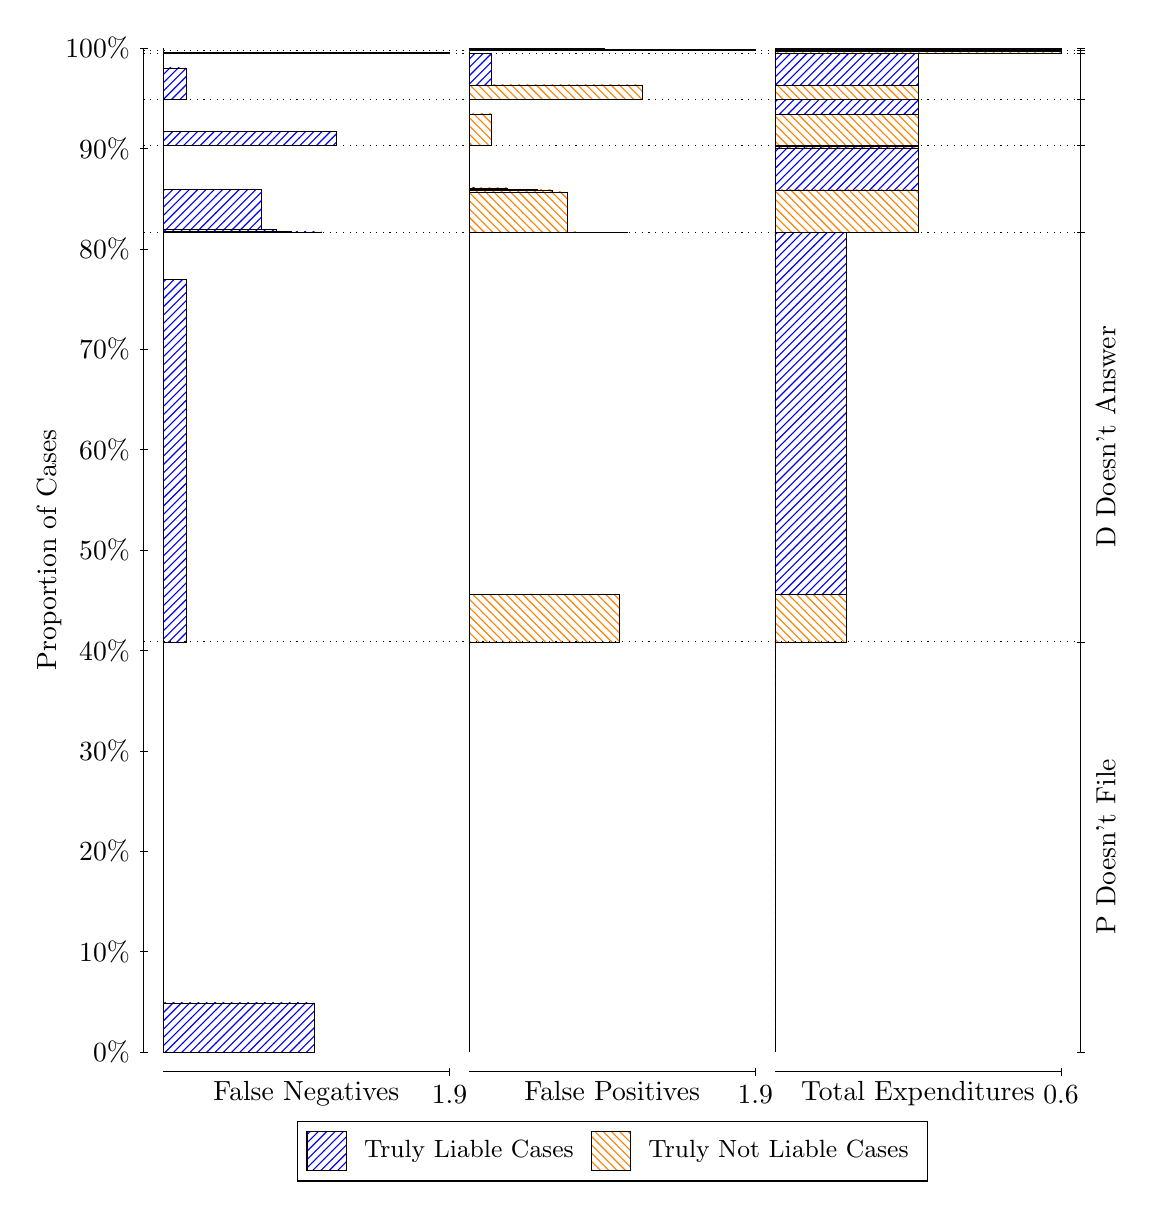
\begin{tikzpicture}
\draw[black, very thin] (1.5,1.75) -- (1.5,14.5);
\node[rotate=90, anchor=center] at (0.3, 8.125) {Proportion of Cases};
\draw[black, very thin] (1.45,1.75) -- (1.55,1.75);
\node[anchor=east] at (1.45, 1.75) {0\%};
\draw[black, very thin] (1.45,3.025) -- (1.55,3.025);
\node[anchor=east] at (1.45, 3.025) {10\%};
\draw[black, very thin] (1.45,4.3) -- (1.55,4.3);
\node[anchor=east] at (1.45, 4.3) {20\%};
\draw[black, very thin] (1.45,5.575) -- (1.55,5.575);
\node[anchor=east] at (1.45, 5.575) {30\%};
\draw[black, very thin] (1.45,6.85) -- (1.55,6.85);
\node[anchor=east] at (1.45, 6.85) {40\%};
\draw[black, very thin] (1.45,8.125) -- (1.55,8.125);
\node[anchor=east] at (1.45, 8.125) {50\%};
\draw[black, very thin] (1.45,9.4) -- (1.55,9.4);
\node[anchor=east] at (1.45, 9.4) {60\%};
\draw[black, very thin] (1.45,10.675) -- (1.55,10.675);
\node[anchor=east] at (1.45, 10.675) {70\%};
\draw[black, very thin] (1.45,11.95) -- (1.55,11.95);
\node[anchor=east] at (1.45, 11.95) {80\%};
\draw[black, very thin] (1.45,13.225) -- (1.55,13.225);
\node[anchor=east] at (1.45, 13.225) {90\%};
\draw[black, very thin] (1.45,14.5) -- (1.55,14.5);
\node[anchor=east] at (1.45, 14.5) {100\%};

\draw[black, very thin] (13.4,1.75) -- (13.4,14.5);
\draw[black, very thin] (13.35,1.75) -- (13.45,1.75);
\node[anchor=west] at (13.35, 1.75) {};
\draw[black, very thin] (13.35,6.9594) -- (13.45,6.9594);
\node[anchor=west] at (13.35, 6.9594) {};
\draw[black, very thin] (13.35,12.161) -- (13.45,12.161);
\node[anchor=west] at (13.35, 12.161) {};
\draw[black, very thin] (13.35,13.265) -- (13.45,13.265);
\node[anchor=west] at (13.35, 13.265) {};
\draw[black, very thin] (13.35,13.847) -- (13.45,13.847);
\node[anchor=west] at (13.35, 13.847) {};
\draw[black, very thin] (13.35,14.434) -- (13.45,14.434);
\node[anchor=west] at (13.35, 14.434) {};
\draw[black, very thin] (13.35,14.471) -- (13.45,14.471);
\node[anchor=west] at (13.35, 14.471) {};
\draw[black, very thin] (13.35,14.5) -- (13.45,14.5);
\node[anchor=west] at (13.35, 14.5) {};

\draw[black, very thin, pattern color=blue, pattern=north east lines] (1.75,1.75) rectangle (3.6623,2.3733);
\draw[black, very thin, pattern color=orange, pattern=north west lines] (1.75,2.3733) rectangle (1.75,6.9594);
\draw[black, very thin, pattern color=blue, pattern=north east lines] (1.75,6.9594) rectangle (2.0368,11.558);
\draw[black, very thin, pattern color=orange, pattern=north west lines] (1.75,11.558) rectangle (1.75,12.161);
\draw[black, very thin, pattern color=blue, pattern=north east lines] (1.75,12.161) rectangle (3.7579,12.165);
\draw[black, very thin, pattern color=blue, pattern=north east lines] (1.75,12.165) rectangle (3.5667,12.165);
\draw[black, very thin, pattern color=blue, pattern=north east lines] (1.75,12.165) rectangle (3.3754,12.168);
\draw[black, very thin, pattern color=blue, pattern=north east lines] (1.75,12.168) rectangle (3.1842,12.194);
\draw[black, very thin, pattern color=blue, pattern=north east lines] (1.75,12.194) rectangle (2.993,12.701);
\draw[black, very thin, pattern color=blue, pattern=north east lines] (1.75,12.701) rectangle (2.8018,12.701);
\draw[black, very thin, pattern color=blue, pattern=north east lines] (1.75,12.701) rectangle (2.6105,12.702);
\draw[black, very thin, pattern color=blue, pattern=north east lines] (1.75,12.702) rectangle (2.4193,12.702);
\draw[black, very thin, pattern color=blue, pattern=north east lines] (1.75,12.702) rectangle (2.2281,12.702);
\draw[black, very thin, pattern color=orange, pattern=north west lines] (1.75,12.702) rectangle (1.75,13.265);
\draw[black, very thin, pattern color=blue, pattern=north east lines] (1.75,13.265) rectangle (3.9491,13.446);
\draw[black, very thin, pattern color=orange, pattern=north west lines] (1.75,13.446) rectangle (1.75,13.847);
\draw[black, very thin, pattern color=blue, pattern=north east lines] (1.75,13.847) rectangle (2.0368,14.248);
\draw[black, very thin, pattern color=orange, pattern=north west lines] (1.75,14.248) rectangle (1.75,14.434);
\draw[black, very thin, pattern color=blue, pattern=north east lines] (1.75,14.434) rectangle (5.3833,14.449);
\draw[black, very thin, pattern color=orange, pattern=north west lines] (1.75,14.449) rectangle (1.75,14.471);
\draw[black, very thin, pattern color=orange, pattern=north west lines] (1.75,14.471) rectangle (1.75,14.485);
\draw[black, very thin, pattern color=blue, pattern=north east lines] (1.75,14.485) rectangle (1.75,14.5);
\draw[black, very thin, pattern color=orange, pattern=north west lines] (5.6333,1.75) rectangle (5.6333,6.3361);
\draw[black, very thin, pattern color=blue, pattern=north east lines] (5.6333,6.3361) rectangle (5.6333,6.9594);
\draw[black, very thin, pattern color=orange, pattern=north west lines] (5.6333,6.9594) rectangle (7.5456,7.5631);
\draw[black, very thin, pattern color=blue, pattern=north east lines] (5.6333,7.5631) rectangle (5.6333,12.161);
\draw[black, very thin, pattern color=orange, pattern=north west lines] (5.6333,12.161) rectangle (7.6412,12.162);
\draw[black, very thin, pattern color=orange, pattern=north west lines] (5.6333,12.162) rectangle (7.45,12.162);
\draw[black, very thin, pattern color=orange, pattern=north west lines] (5.6333,12.162) rectangle (7.2588,12.163);
\draw[black, very thin, pattern color=orange, pattern=north west lines] (5.6333,12.163) rectangle (7.0675,12.164);
\draw[black, very thin, pattern color=orange, pattern=north west lines] (5.6333,12.164) rectangle (6.8763,12.672);
\draw[black, very thin, pattern color=orange, pattern=north west lines] (5.6333,12.672) rectangle (6.6851,12.698);
\draw[black, very thin, pattern color=orange, pattern=north west lines] (5.6333,12.698) rectangle (6.6851,12.698);
\draw[black, very thin, pattern color=orange, pattern=north west lines] (5.6333,12.698) rectangle (6.4939,12.704);
\draw[black, very thin, pattern color=orange, pattern=north west lines] (5.6333,12.704) rectangle (6.3026,12.705);
\draw[black, very thin, pattern color=orange, pattern=north west lines] (5.6333,12.705) rectangle (6.1114,12.724);
\draw[black, very thin, pattern color=blue, pattern=north east lines] (5.6333,12.724) rectangle (5.7289,12.724);
\draw[black, very thin, pattern color=blue, pattern=north east lines] (5.6333,12.724) rectangle (5.6333,13.265);
\draw[black, very thin, pattern color=orange, pattern=north west lines] (5.6333,13.265) rectangle (5.9202,13.665);
\draw[black, very thin, pattern color=blue, pattern=north east lines] (5.6333,13.665) rectangle (5.6333,13.847);
\draw[black, very thin, pattern color=orange, pattern=north west lines] (5.6333,13.847) rectangle (7.8325,14.033);
\draw[black, very thin, pattern color=blue, pattern=north east lines] (5.6333,14.033) rectangle (5.9202,14.434);
\draw[black, very thin, pattern color=orange, pattern=north west lines] (5.6333,14.434) rectangle (5.6333,14.456);
\draw[black, very thin, pattern color=blue, pattern=north east lines] (5.6333,14.456) rectangle (5.6333,14.471);
\draw[black, very thin, pattern color=orange, pattern=north west lines] (5.6333,14.471) rectangle (9.2667,14.485);
\draw[black, very thin, pattern color=blue, pattern=north east lines] (5.6333,14.485) rectangle (7.3544,14.5);
\draw[black, very thin, pattern color=orange, pattern=north west lines] (9.5167,1.75) rectangle (9.5167,6.3361);
\draw[black, very thin, pattern color=blue, pattern=north east lines] (9.5167,6.3361) rectangle (9.5167,6.9594);
\draw[black, very thin, pattern color=orange, pattern=north west lines] (9.5167,6.9594) rectangle (10.425,7.5631);
\draw[black, very thin, pattern color=blue, pattern=north east lines] (9.5167,7.5631) rectangle (10.425,12.161);
\draw[black, very thin, pattern color=orange, pattern=north west lines] (9.5167,12.161) rectangle (11.333,12.698);
\draw[black, very thin, pattern color=blue, pattern=north east lines] (9.5167,12.698) rectangle (11.333,13.231);
\draw[black, very thin, pattern color=orange, pattern=north west lines] (9.5167,13.231) rectangle (11.333,13.251);
\draw[black, very thin, pattern color=blue, pattern=north east lines] (9.5167,13.251) rectangle (11.333,13.254);
\draw[black, very thin, pattern color=orange, pattern=north west lines] (9.5167,13.254) rectangle (11.333,13.261);
\draw[black, very thin, pattern color=blue, pattern=north east lines] (9.5167,13.261) rectangle (11.333,13.265);
\draw[black, very thin, pattern color=orange, pattern=north west lines] (9.5167,13.265) rectangle (11.333,13.665);
\draw[black, very thin, pattern color=blue, pattern=north east lines] (9.5167,13.665) rectangle (11.333,13.847);
\draw[black, very thin, pattern color=orange, pattern=north west lines] (9.5167,13.847) rectangle (11.333,14.033);
\draw[black, very thin, pattern color=blue, pattern=north east lines] (9.5167,14.033) rectangle (11.333,14.434);
\draw[black, very thin, pattern color=orange, pattern=north west lines] (9.5167,14.434) rectangle (13.15,14.456);
\draw[black, very thin, pattern color=blue, pattern=north east lines] (9.5167,14.456) rectangle (13.15,14.471);
\draw[black, very thin, pattern color=orange, pattern=north west lines] (9.5167,14.471) rectangle (13.15,14.485);
\draw[black, very thin, pattern color=blue, pattern=north east lines] (9.5167,14.485) rectangle (13.15,14.5);
\draw[black, dotted] (1.5,6.9594) -- (13.4,6.9594);
\draw[black, dotted] (1.5,12.161) -- (13.4,12.161);
\draw[black, dotted] (1.5,13.265) -- (13.4,13.265);
\draw[black, dotted] (1.5,13.847) -- (13.4,13.847);
\draw[black, dotted] (1.5,14.434) -- (13.4,14.434);
\draw[black, dotted] (1.5,14.471) -- (13.4,14.471);
\draw[black, very thin] (1.75,1.5) -- (5.3833,1.5);
\node[anchor=north] at (3.5667, 1.5) {False Negatives};
\draw[black, very thin] (5.3833,1.45) -- (5.3833,1.55);
\node[anchor=north] at (5.3833, 1.45) {1.9};

\draw[black, very thin] (5.6333,1.5) -- (9.2667,1.5);
\node[anchor=north] at (7.45, 1.5) {False Positives};
\draw[black, very thin] (9.2667,1.45) -- (9.2667,1.55);
\node[anchor=north] at (9.2667, 1.45) {1.9};

\draw[black, very thin] (9.5167,1.5) -- (13.15,1.5);
\node[anchor=north] at (11.333, 1.5) {Total Expenditures};
\draw[black, very thin] (13.15,1.45) -- (13.15,1.55);
\node[anchor=north] at (13.15, 1.45) {0.6};

\node[black, centered, rotate=90] at (13.72, 4.3547) {P Doesn't File};
\node[black, centered, rotate=90] at (13.72, 9.5604) {D Doesn't Answer};






\draw (7.449999999999999,1.5) node[draw=none] (baseCoordinate) {};
\begin{scope}[align=center]
        \matrix[scale=0.5, draw=black, below=0.5cm of baseCoordinate, nodes={draw}, column sep=0.1cm]{
            \node[rectangle, draw, minimum width=0.5cm, minimum height=0.5cm, pattern=north east lines, pattern color=blue] {}; &
            \node[draw=none, font=\small] (B) {Truly Liable Cases}; &
            \node[rectangle, draw, minimum width=0.5cm, minimum height=0.5cm, pattern=north west lines, pattern color=orange] {}; &
            \node[draw=none, font=\small] (B) {Truly Not Liable Cases}; \\
            };
\end{scope}

\end{tikzpicture}
\end{document}